
\section{La Web Semántica}

En 1989 Tim Berners-Lee realizó para el CERN un modelo de gestión de la 
información basado en un sistema distribuido de hipertexto\footnote{\url{http://www.w3.org/Proposal}}. 
Fue el origen de lenguaje de marcado HTML y la semila de la Web actual
que recientemente ha cumplido 15 años\footnote{\url{http://www.sun.com/aboutsun/media/features/www15.html}}.

No tardó mucho en darse cuenta que ese modelo no era suficiente para 
manejar grandes volúmenes de información, pues resultaría muy dificil 
encontrarla y usarla eficientemente. Así el propio Tim Berners-Lee 
expondría\footnote{\url{http://www.scientificamerican.com/article.cfm?articleID=00048144-10D2-1C70-84A9809EC588EF21&catID=2}}
en 2001 su visión\footnote{Cita extraida de las transparencias de José Emilio 
Labra Gayo para el curso de verano sobre Web Semántica de la Universidad de 
Oviedo, \url{http://www.di.uniovi.es/~labra/cursos/ver06/}} de la Web Semántica:

\begin{quote}
	\emph{«... \textbf{disponer datos} en la Web \textbf{definidos y enlazados} 
	de forma que puedan ser \textbf{utilizados por las máquinas}, no solamente 
	para visualizarnos, sino también para \textbf{automatizar} tareas, 
	\textbf{integrar} y \textbf{reutilizar} datos entre aplicaciones.»}
\end{quote} 

Y quizás se está dedicando mucho esfuerzo a publicar y procesar de forma autónoma
esos datos, obviando quizás la parte más importante: 
\textbf{enlazarlos}\footnote{Traducción libre de un extracto de un documento (\url{http://www.w3.org/DesignIssues/LinkedData}) de Tim Berners-Lee}.

\begin{quote}
	\emph{«La Web Semántica no sólo se trata de publicar datos en la Web. Se 
	trata de enlazarlos para que personas o máquinas podamos explorar esos 
	datos. Al estar enlazados, podremos encontrar fácilmente datos relacionados 
	con los datos que disponemos.»}
\end{quote}

\subsection{Evolución de la Web}

La Web es un recurso muy especial y particular, con unas características muy 
especiales que deben tenerse en cuenta: no centralizada, información dinámica,
mucha cantidad de información y está abierta a todo el mundo.

En los últimos años la Web ha experimentado una notable evolución, como puede 
verse en la figura \ref{fig:evoWeb}\footnote{Extraida de una presentación 
(\url{http://www.w3c.es/Presentaciones/2005/1018-WebSemanticaREBIUN-MA/}) de 
Martín Álvarez Espinar, de la Oficina Española del W3C}, que le ha llevado a 
convertirse no sólo en un almacen de contenido estático, sino también en un 
repositorio universal de conocimiento y servicios.

\begin{figure}[ht]
	\centering
	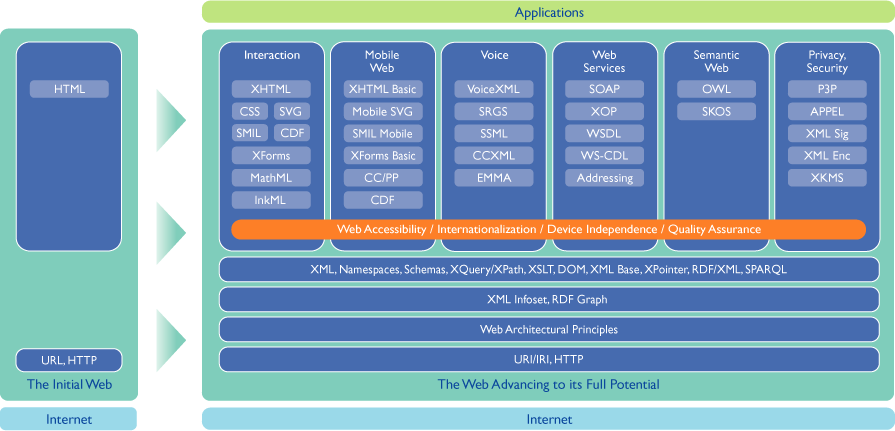
\includegraphics[width=12cm]{images/web-evolution.png}
	\caption{Evolución de la Web}
	\label{fig:evoWeb}
\end{figure}

A pesar de todas estas pequeñas revoluciones, todavia seguimos en una web 
\emph{sintáctica}. Una Web en la que todavía es muy difícil realizar
muchas tareas que con la Web Semántica, y todas sus tecnologías, al menos
serán un poco más fácil de hacer.

\subsection{Estructura de la Web Semántica}

La Web Semántica se encuentra estructurada en capas (la llamada \emph{tarta de 
la Web Semántica}), de forma que se pudiera trabajar en cada uno de estos
sustratos de manera independiente a el estado de la implementación de las
capas inferiores y/o superiores.

Algunas parte del diseño aún se estan discutiendo en los distintos grupos de
trabajo, aunque en la figura \ref{fig:swStack} encontramos el diseño que toma
más forma después de los últimos años de trabajo:

\begin{figure}[ht]
	\centering
	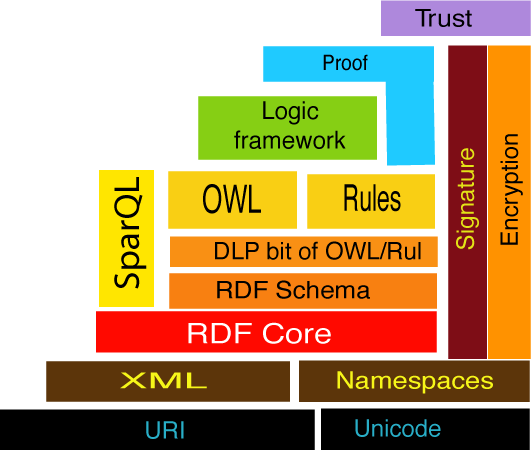
\includegraphics[width=10cm]{images/semantic-web-stack.png}
	\caption{Pila de la web semántica}
	\label{fig:swStack}
\end{figure}

Puede verse que el nucleo de la Web Semántica se fundamenta sobre tres 
tecnologías fundamentales:

\begin{itemize}
  \item RDF
  \item OWL
  \item SPARQL
\end{itemize}

Con una envoltura de lógica y reglas, sustentadas sobre una infraestructura 
basada en XML, URI's y Unicode.

Veáse que las reglas pasan a estar a mismo nivel que las ontologías, y no por
encima como se pensaba en los primeros diseños, por la íntima relación que ambas
tienen.

\subsection{Elementos}

\subsubsection{Elementos básicos}

\paragraph{Unicode}

Unicode\footnote{\url{http://www.unicode.org/}} es una iniciativa de un consorcio de 
empresas dedicadas a la internacionalización para conseguir una representación 
informática de los caracteres en todos los idiomas de forma que pueda ser representados
y manipulados de forma universal. 

Aunque existen varias codificaciónes distintas, 
UTF-8\footnote{\url{http://www.ietf.org/rfc/rfc3629.txt}} es la codificación 
unicode más usada y extendida, tanto por su sencillez (usa grupos de bytes) 
como por su flexibilidad (los alfabetos de muchos de los lenguajes del mundo 
se pueden representar en UTF-8).

Unicode es el recurso primario de representación de caracteres en la Web Semántica.

\paragraph{URI}

Acronimo del inglés Uniform Resource Identifier, identificador uniforme de recursos.
Mecanismo que la Web Semántica utiliza para identificar recursos. 

Un concepto que mezcla URL\footnote{Uniform Resource Locator, localizador uniforme de recurso} 
y URN\footnote{Uniform Resource Name, nombre uniforme de recurso} para cumplir una doble 
funcionalidad: servir como protocolo de acceso e identificar de manera única los recursos 
en la World Wide Web.

\subsubsection{XML}

XML\footnote{\url{http://www.w3.org/XML/}} (eXtensible Markup Language, Lenguaje 
de marcado extensible) es un formato de marcado estructurado para la representación 
de información muy usado y extendido hoy en día, hasta tal punto de ser considerado 
el lenguaje universal para el intercambio de información. 

Desarrollado por el W3C a partir de SGML\footnote{\url{http://www.w3.org/MarkUp/SGML/}} 
con el objetivo que fuera fácilmente procesable por una máquina y legible por un 
humano. 

Basandose en una definición abstracta (XML Schema), permite extender su gramática 
de una forma muy fácil y sencilla de procesar (XSL/XSLT, XPath, XPoint, etc).

Es usado en múltiples tecnológías hoy en día, sobre todo en la web (XHTML, XForms, 
SVG, etc), aunque también para documentación (DocBook), interfaces de usuario (XUL,
Glade, XAML, etc), protocolos (Jabber), etc. Se utilizan espacios de nombres (namespace), 
identificados por URI's, para mezclar en un documento etiquetas pertenecientes a 
diferentes vocabularios.

Pero XML, a pesar de ser un lenguaje estructurado que es muy fácil de procesar, 
aún carece de la semántica necesaria. 

Sobre XML existe mucha bibliografia relacionada, siendo recomenable empezar por
\emph{XML Imprescindible}\cite{XMLNutshell}, un excelente libro que hace un amplio
recorrido por XML y todas sus tecnologías.

\subsubsection{RDF}

Acrónimo del inglés \emph{Resource Description Framework} (marco de descripción 
de recursos), RDF\footnote{\url{http://www.w3.org/RDF/}} es una especificación del 
W3C originalmente diseñada como modelo de datos, pero su uso se ha extendido como
método general para modelar el conocimiento.

RDF es un modelo de tripletas del tipo \texttt{(sujecto, predicado, objecto)}. El
sujeto es un recurso que se identifica con una URI, y se relaciona mediante un 
predicado binario con el objeto, que puede ser otra URI o un literal.

\begin{figure}[ht]
	\centering
	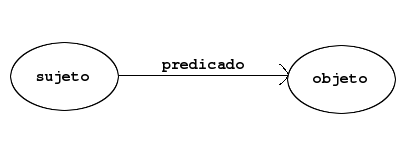
\includegraphics[width=10cm]{images/arc.png}
	\caption{Arco RDF}
	\label{fig:rdfTriplet}
\end{figure}

Cada tripleta puede verse como un arco, que al juntarse con otros arcos se obtiene
un grafo dirigido que describe los recursos y las relaciones entre todos los 
recursos.

Un ejemplo sencillo: \textit{Sergio Fdez es el creador de http://www.wikier.org/}. 
Usando Dublin Core (sección \ref{sec:dc}) podría quedar la siguiente tripleta: 
\texttt{(http://www.wikier.org/, dc:creator, "Sergio Fdez")}. Dando lugar a un 
grafo del estilo de:

\begin{figure}[ht]
	\centering
	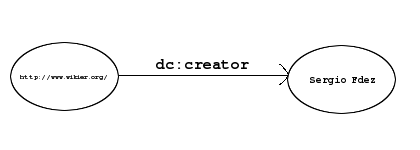
\includegraphics[width=10cm]{images/arc-example.png}
	\caption{Ejemplo de arco RDF}
	\label{fig:rdfTripletExample}
\end{figure}


RDF se puede serializar con tres sintáxis: en XML, N3 (notación de tripletas)
o Turtle. El mismo grafo se podría serializar con las dos sintáxis, conteniendo ambos 
idéntica información semántica:

\begin{figure}
\begin{verbatim}
	<rdf:RDF xmlns:rdf="http://www.w3.org/1999/02/22-rdf-syntax-ns#"
	         xmlns:rdfs="http://www.w3.org/2000/01/rdf-schema#"
                 xmlns:dc="http://purl.org/dc/elements/1.1/"
	>
	  <rdf:Description rdf:about="http://www.wikier.org/">
	    <dc:creator>Sergio Fdez</dc:creator>	
	  </rdf:Description>
	</rdf:RDF>
\end{verbatim}
	\caption{Ejemplo de grafo RDF serializado en XML}
	\label{fig:ejemplo.rdfxml}
\end{figure}

\begin{figure}
\begin{verbatim}
	@prefix dc <http://http://purl.org/dc/elements/1.1/>
	<http://www.wikier.org> dc:creator "Sergio Fdez"
\end{verbatim}
	\caption{Ejemplo de grafo RDF serializado en N3}
	\label{fig:ejemplo.rdfn3}
\end{figure}

\begin{figure}
\begin{verbatim}
	@prefix dc <http://http://purl.org/dc/elements/1.1/>
	<http://www.wikier.org> 
		dc:creator "Sergio Fdez"
\end{verbatim}
	\caption{Ejemplo de grafo RDF serializado en Turtle}
	\label{fig:ejemplo.rdfturtle}
\end{figure}

\subsubsection{RDFS}

RDFS\footnote{\url{http://www.w3.org/TR/rdf-schema/}} (RDF Schema) es una
forma primitiva y limitada de describir ontologías en RDF, también llamado
«\emph{vocabulario RDF}».

\subsubsection{OWL}

Del acrónimo en inglés \emph{Ontology Web Languaje}, 
OWL\footnote{\url{http://www.w3.org/TR/owl-features/}} es la recomendación 
oficial de W3C\footnote{\url{http://www.w3.org/}} para publicar ontologías en 
la Web. Se trata de un lenguaje de gran expresividad para describir conceptos 
y relaciones entre conceptos, con un compromiso entre expresividad y tratabilidad

Tiene en DAML+OIL\footnote{\url{http://www.daml.org/2001/03/daml+oil-index}}, 
otros dos lenguajes de ontologías, sus antecesores inmediatos.

La versión actual de OWL (1.0) tiene principalmente tres variantes según su
complejidad:

\begin{itemize}
  \item OWL Full, intimamente ligado a la lógica de RDF, pero que puede resultar
	no computable.
  \item OWL DL, un subconjunto del anterior basado en la lógica descriptiva 
	\begin{displaymath}
		{SHOIN} (D)
	\end{displaymath}
  \item OWL Lite, subconjunto de OWL DL que se basa en la lógica menos descriptiva
	\begin{displaymath}
 		{SHIF} (D)
	\end{displaymath}
\end{itemize}

Una perpectiva sencilla sería mostrada por la figura \ref{fig:owlVariants}.

\begin{figure}[ht]
	\centering
	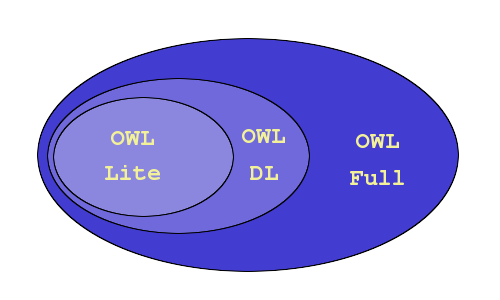
\includegraphics[width=12cm]{images/owl-variants.png}
	\caption{Perspectiva completa de OWL}
	\label{fig:owlVariants}
\end{figure}

Aunque el panorama no es tan sencillo, y para diferenciar cada una de ellas no
se puede hacer fijandose sólo en la complejidad, sino también en la parte de la 
lógica que abarcan. Quedando un panorama aún más confuso, como se puede ver en 
la figura \ref{fig:owlVariantsExtended}\footnote{Gráfico extraido de Ontotext, 
\url{http://www.ontotext.com/inference/rdfs_rules_owl.html#owl_fragments}}.

\begin{figure}[ht]
	\centering
	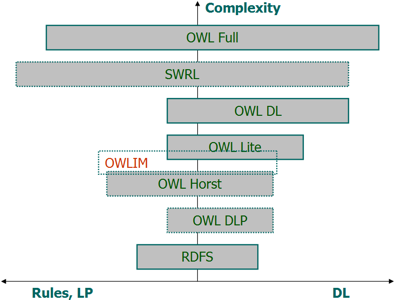
\includegraphics[width=10cm]{images/owl-dialects.png}
	\caption{Variantes de OWL ampliado}
	\label{fig:owlVariantsExtended}
\end{figure}

Hay que tener en cuenta que existe cierto solapamiento entre la expresividad de
OWL y la de RDFs (RDF-Schema), desvirtuando en cierta manera la visión original
por capas.

Para más información puede consultarse el último libro publicado de OWL\cite{OWL} 
que yo he encontrado.

\subsubsection{SPARQL}

SPARQL\footnote{\url{http://www.w3.org/TR/rdf-sparql-query/}} es un nuevo lenguaje,
uno de tantos\cite{ComparisonRDFQuery}, de consulta sobre la base del conocimiento 
en OWL/RDF con un compromiso en su justa medida entre semántica y 
complejidad\cite{SemanticsComplexitySPARQL}. Actualmente se trata del candidato a 
recomendación del W3C por parte del 
DAWG\footnote{\url{http://www.w3.org/2001/sw/DataAccess/}} (RDF Data Access Working 
Group).

Posee una sintáxis similar a la otros lenguajes de consulta relacionales, como
podría ser SQL. De hecho sus algebras comparten\cite{RelationalAlgebraSPARQL} 
determinados puntos. 

\begin{figure}[ht]
	\begin{verbatim}
		PREFIX rdf: <http://www.w3.org/1999/02/22-rdf-syntax-ns#>
		PREFIX dc: <http://purl.org/dc/elements/1.1/>
		SELECT DISTINCT ?x, ?name
		WHERE {
		  ?x dc:creator ?name
		}
	\end{verbatim}
	\centering
	\caption{Ejemplo de consulta SPARQL}
	\label{fig:ejemplo.sparql}
\end{figure}

Aplicando esta sencilla consulta de ejemplo a un RDF, como por ejemplo el de 
antes \ref{fig:ejemplo.rdfxml}, se obtendría el nombre del creador de cada recurso
definido.

A pesar de ser un lenguaje relativamente reciente, ya se encuentran disponibles
API's de consulta para numerosos lenguajes de programación: 
RDFLib\footnote{\url{http://rdflib.net/sparql/}} para Python, 
Jena\footnote{\url{http://jena.sourceforge.net/ARQ/}} en Java, 
Redland RDF\footnote{\url{http://librdf.org/}} en C con bindings también para 
otros lenguajes, twinql\footnote{\url{http://www.holygoat.co.uk/projects/twinql/}} 
en Lisp,etc. Además de estar soportado por alguno de los razonadores más conocidos, 
como Pellet\footnote{\url{http://www.mindswap.org/2003/pellet/}} o 
KAON2\footnote{\url{http://kaon2.semanticweb.org/}}.

\subsection{Aplicaciones prácticas}

\subsubsection{Vocabularios RDF}

Existen multitud de vocabularios RDF para fines muy concretos, desde describir
personas, hasta eventos. Estos vocabularios suelen ser fácilmente extensibles y 
reutilizables entre si.

Existen multitud de ejemplos:

\paragraph{Dublin Core\label{sec:dc}}

Dublin Core\footnote{\url{http://dublincore.org/}}, también conocido por sus siglas DC,
es un vocabulario RDF para la descripción de múltiples propiedades de todo tipo de 
recursos online.

\paragraph{RSS}

Desarrollado en el seno de Netscape, RSS es el formato de sindicación de noticias
más extendido en la actualidad. Con un complicado historial de versiones\ref{fig:rssEvolution} 
incompatibles entre sí (sólo la versión 1.0 de RSS sean
RDF, el resto de versiones 

\begin{figure}[ht]
	\centering
	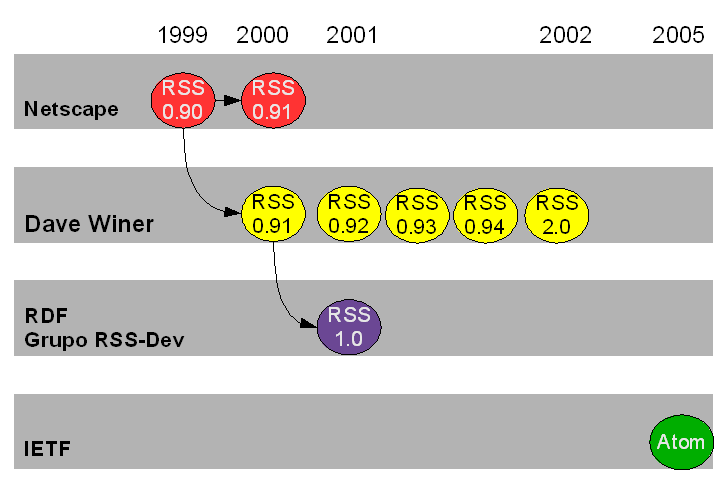
\includegraphics[width=10cm]{images/rssEvolution.png}
	\caption{Evolucion de RSS}
	\label{fig:rssEvolution}
\end{figure}

\paragraph{FOAF}

FOAF\footnote{\url{http://www.foaf-project.org/}}, acrónimo de Friend-of-a-Friend, 
se trata de un vocabulario RDF para describir semánticamente información personal
muy extendido (en 2004 se estimaba\cite{Li2005} que existian alrededor de 1,2 millones 
de documentos FOAF) dentro del ámbito de la web semántica.

\begin{figure} [ht]
\begin{verbatim}
	<rdf:RDF
		xmlns:rdf="http://www.w3.org/1999/02/22-rdf-syntax-ns#"
		xmlns:rdfs="http://www.w3.org/2000/01/rdf-schema#"
		xmlns:foaf="http://xmlns.com/foaf/0.1/"
	>
	  <foaf:Person rdf:nodeID="me">
	    <foaf:name>Sergio Fernández</foaf:name>
	    <foaf:title>Mr</foaf:title>
	    <foaf:firstName>Sergio</foaf:firstName>
	    <foaf:surname>Fernández</foaf:surname>
	    <foaf:gender>Male</foaf:gender>
	    <foaf:mbox>sergio@wikier.org</foaf:mbox>
	  </foaf:Person>
	</rdf:RDF>
\end{verbatim}
	\caption{Ejemplo de FOAF}
	\label{fig:ejemplo.foaf}
\end{figure}

\begin{figure}
 	\centering
	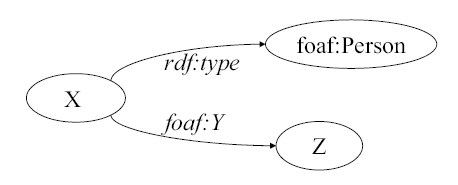
\includegraphics[width=7cm]{images/patron-foaf.png}
	\caption{Patrón de documentos FOAF}
	\label{fig:patternFOAF}
\end{figure}

Pudiendo describir relaciones (amigos, compañeros de trabajo, etc), interéses,
proyectos y demás recursos de uso personal, de forma que se forme un grafo 
uniendo todos ellos. El patrón\ref{fig:patternFOAF} siempre se repite.

\paragraph{DOAP}

Description-of-a-Project\footnote{\url{http://usefulinc.com/doap}} es una idea 
similar a FOAF pero para describir proyectos de software libre.

\begin{figure}[ht]
\begin{verbatim}

<rdf:RDF xmlns:rdf="http://www.w3.org/1999/02/22-rdf-syntax-ns#" 
         xmlns:rdfs="http://www.w3.org/2000/01/rdf-schema#" 
         xmlns:doap="http://usefulinc.com/ns/doap#" 
         xmlns:foaf="http://xmlns.com/foaf/0.1/" 
         xmlns:admin="http://webns.net/mvcb/" 
         xml:lang="en">

  <doap:Project rdf:about="http://swaml.berlios.de/">

    <doap:name>Semantic Web Archive of Mailing Lists</doap:name>
    <doap:shortname>SWAML</doap:shortname>

    <doap:homepage rdf:resource="http://swaml.berlios.de/"/>
    <doap:created>2005-09-24</doap:created>

    <doap:description xml:lang="en">
      SWAML is a research project around the semantic web tecnologies 
      to publish the mailing lists's archive into an RDF format.
    </doap:description>
    <doap:description xml:lang="es">
      SWAML es un proyecto de investigación alrededor de las tecnologías 
      de la web semántica para publicar los archivos de las listas de 
      correo en un formato RDF.
    </doap:description>

    <doap:wiki rdf:resource="http://swaml.berlios.de/wiki"/>
    <doap:bug-database rdf:resource="http://swaml.berlios.de/bugs"/>
    <doap:programming-language>python</doap:programming-language>
    <doap:license rdf:resource="http://usefulinc.com/doap/licenses/gpl"/>
    <doap:download-page rdf:resource="http://swaml.berlios.de/#files"/>
    <doap:download-mirror rdf:resource="http://swaml.berlios.de/files"/>

  </doap:Project>

</rdf:RDF>
\end{verbatim}
	\caption{Fichero DOAP de SWAML}
	\label{fig:ejemplo.doap}
\end{figure}

\paragraph{EARL}

FIXME

\subsubsection{Otras aplicaciones de RDF}

\paragraph{Mozilla}

FIXME

\subsection{Libros de interés}

Aunque no existen buenas publicaciones en castellano, hay varios libros en inglés 
que es imprescindible ojear: \emph{A Semantic Web primer}\cite{SemanticWebPrimer},
\emph{Practical RDF}\cite{PracticalRDF}, 
\emph{Spinning the Semantic Web}\cite{SpinningSemanticWeb}
\emph{Explorer's Guide to the Semantic Web}\cite{ExplorerSemanticWeb}.

\subsection{Futuro}

Hacia donde irá la Web Semántica es algo que sólo se sabrá con el tiempo, y quizás
en un plazo no más allá de 5 o 10 años. Por ahora es muy pronto para aventurar nada,
aunque si bien es cierto que el estado de adopción de la Web Semántica, en palabras
del propio Ivan Herman\footnote{\url{http://www.w3.org/2006/Talks/1109-Athens-IH/}},
crece a un ritmo imparable.

Históricamente todos los campos relacionados con la IA (inteligencia artificial) 
han sido áreas de investigación vendidas en exceso como la panacea de la solución 
de todos los problemas de la humanidad; generando unas espectativas falsas que han 
hecho mucho daño a la comunidad científica.

Lo que si sabemos es que la Web Semántica será una Web mucho más \emph{útil}.
